%************************************************
%\chapter{A model for distributed web-based human- and machine-driven computation}
\chapter{Conceptual model}
\label{cap:model}
%************************************************



In this chapter it is presented a framework for task distribution and execution
able to cover all the dimension defined in \autoref{tab:matrix}.
First there is introduced a methodology to follow in order to pass from the model to the
actual application implementation, available in \autoref{cap:implementation}.
The components that will compose the framework are founded on a data model,
describing the logical structure of the data processed by the application.

The data model is composed of three parts: the \emph{Data Model}, the
\emph{Architectural Model} and the \emph{Execution model}. Eventually there are
explained the pluggable strategies available for this framework.
\begin{description}
    \item[The Data Model] describes the data structures
    used to support the framework.
    \item[The Architectural Model] describes
    the reference architecture of the framework.
    \item[The Execution Model] focuses on the
    execution model of the task.
    \item[The Pluggable Strategies] describes
    the possible configuration points of the framework.
\end{description}

\section{Development methodology}
\label{sec:model:method}
% TODO ??

During the development process of \myTitle the first issue that need to be
resolved was the description of a suitable model for supporting such framework.
The design of a model involves the definition of the data structures that will
be used by the workflow, and of course the definition of the workflow itself.

\subsection{Data Design}
% durante il design abbiamo dovuto tener conto del problema che dovevamo risolvere
% data la flessibilità e generalità di questo 
% abbiamo desciso di usare un metamodello
% il metamodello voveva essree in grasdo di supportare i processi descritti più avanti
%  pluggabilità
In the design process for the data model we faced the problem of creating a
suitable underlying model for all the application need that we have to cover,
spacing from pure \acl{HC} task to \emph{parasitic computing}. This wide range
of possible application and the need of great flexibility demanded to the system,
led us to the creation of a meta model for almost all the data structures used in
the framework. The metamodel was subdivided in four: the \emph{Workflow}, the
\emph{Task Data Model}, the \emph{Task Model} and the \emph{Task Execution Model}.

\paragraph{The Workflow Model} describes the flow of the execution of the Task
within the framework, the relationships that needs to be taken into account to
correctly execute a sequence of task (called \emph{Work}).

\paragraph{The Task Data Model} describes the data model for each Task, including,
if present, the field dependencies and if a field belongs to the input or the
output set.

\paragraph{The Task Model} describes the actual data of the Task, called
\emph{Objects}, for the Task.

\paragraph{The Task Execution Model} describes the actual execution step for
each Task, providing information on which user is performing which task, as long
as data associated to the execution itself.


\subsection{Workflow Design}
\begin{figure}[htb]
    \centering
    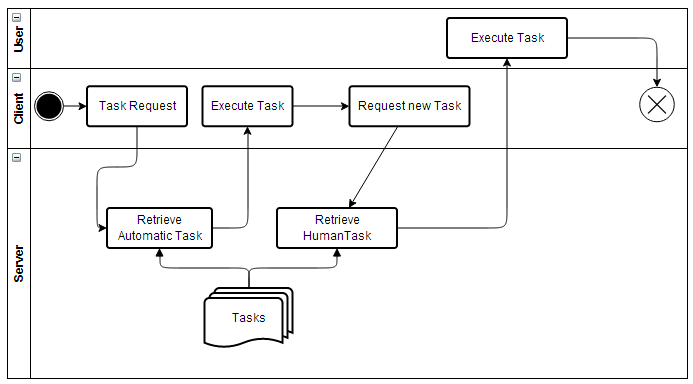
\includegraphics[width=\columnwidth]{Workflow}
    \caption{The conceptual Workflow handled by the framework.}
    \label{fig:workflow}
\end{figure}
% 
In the \emph{Workflow Design} we must describe, at conceptual level, how our
framework deal with the client and how the task are executed. During the
\emph{Data Design} we stated that the tasks can have relationships and thus our
framework must be able to handle different Task types seamlessly. In
\autoref{fig:workflow} is depicted a typical flow of execution of a Work (a
composition of task) with multiple task types.\\

Our Workflow model must be able to handle the interleaving of human and automatic
task without any human intervention. The Workflow must take into account also the
constraints defined during the creation step and manage the execution of the
tasks accordingly.

A feature that the framework is required to handle is also the case where
the application type is not strictly human or strictly automatic. We can have
scenarios where the task is a blend of both human and automatic interactions.
\ac{GWAP} are a case where the automatic computation and the human interaction
are blended together. Other scenarios can be the validation of the automatically
computed results as we presented in our use case (see \ref{sec:cases:hybrid}).

To guarantee the needed flexibility the framework must be able to include third-part
logic in charge of managing certain steps of the execution (like Task planning).




\subsection{Framework Design}
% come sono arrivato all'architettura del framework
In the design of the framework all the conceptual designed data and workflows as
long as the requirements are merged and adapted to create the whole structure for
supporting the framework.\\

During the \textbf{Data Design} we pointed out what are the data structures that
need to be managed. The \emph{Workflow Model} need to specify the relationship
between the modules an the "connection points" where the third part softwares
are plugged. On top of that every Task must have defined its set of input and
output data.
The \emph{Task Data Model} specifies all the data structure of the task, building
the metamodel for each Task. The metamodel contain all the information on the 
structure of the data model for a Task.
In the \emph{Task Model} are contained all the actual data for each Task, called
Objects, each object represents a "row" of the data. Each object is, in turn,
associated to a Task.
The \emph{Task Execution Model} contains all the information on the actual
execution of a Task, keeping information on the user that performer the task and
the used device, if any.\\

The \textbf{Workflow Design} allow us to create the software able to handle all
the different types of archetype application (e.g. Human computation, Automatic
computation) giving also the guidelines on how to manage the interaction between
subsequent Task execution.

\section{Data model}
\label{sec:model:data}
% Data Model
data model


% task con custom proiperties in modo da configurare i runtime

\section{Architectural model}
\label{sec:model:architecture}
\begin{figure}[htb]
	\centering
	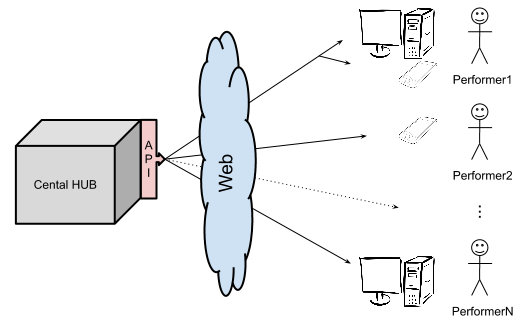
\includegraphics[width=0.75\columnwidth]{Architecture}
	\caption{Reference architecture.}
	\label{fig:architecture}
\end{figure}
% TODO nell'immagine metto anche un dispositivo mobile e un utente con 2 device

During the Design Process we faced the problem of finding a suitable Architectural
Model able to support all the requirements, in terms of flexibility and pluggability,
raised during the Process Design. In our model we use as a reference architecture
the one depicted in \autoref{fig:architecture}. Here we have a central hub
in charge of distributing the Tasks to the nodes\footnote{We refer to nodes
because we want to enclose both humans and devices.} and an abstraction layer.

The \emph{Central Hub} is used to manage all the data exchange between to the
nodes and the hub itself, orchestrating all the communication flow.

The \emph{Abstraction Layer} is used to normalize the differences between the
nodes, creating a coherent representation of nodes.\\




As described in \ref{design:work}, our framework has multiple configuration
points used to customize the Task behavior. As described in \vref{data:task},
for each Task we identified seven configuration points:
\begin{description}
	\item[\utask{} planning strategy:] defines how many \utask{} to create for
	each Task and associate the right portion of Objects to each of them.
	\item[\utask{} implementation strategy:] defines the logic behind the choice
	of a \utask{} implementation sent to a user.
	\item[Performer assignment strategy:] in charge of choosing the users who
	are suitable to execute a certain Task.
	\item[Task Planning strategy:] orchestrates the invocation of the \utask{}
	planning strategy, the \utask{} implementation strategy and the Performer
	assignment strategy.
	\item[Task Control strategy:] defines a controller for the Task, able to
	check the status, and if needed, perform corrective actions.
	\item[Aggregation function:] is in charge of joining the results obtained
	from the \utask{}s execution and create a Task output.
	\item[Emission policy:] is used to rule notifications sent to the Subscribers.
\end{description}
All these configuration points are described in \ref{sec:model:strategies}.

\section{Execution model}
\label{sec:model:execution}
% Execution model
Execution model

\section{Pluggable strategies assignment}
\label{sec:model:strategies}
%% Pluggable+Strategies

As pointed out during the Process Design and briefly introduced in the 
Architectural Model, our framework must be able to handle custom strategies.
These strategies (see \ref{sec:model:architecture}) are used to grant that
our model is flexible enough to support all the application archetypes
defined in \autoref{tab:matrix}.

This section explains the purposes of each strategy and what are the
main properties for each strategy.


\subsection{\utask{} Planning strategy}
The \utask{} Planning strategy is a pluggable logic devoted to the creation, or
deletion, of \utask{}. Eventually this strategy must, during the creation
time of a \utask{}, bind a corresponding set of Task Objects to the \utask{}.
This binding produce a set of \utask{} with the corresponding Task Objects. A
Task planning strategy is defined by:
\begin{itemize}
    \item A set of \textbf{Constraints} that rules the execution.

    \item A \textbf{Planning policy} that can be defined at:
        \begin{description}
            \item[Design time:] the assignment is made at design time during the
            creation phase. After the planning is done it can be modified only

            \item[Dynamic:] the planning is done at least once, using a provided
            set of input \emph{Object}s. The planning can be further invoked due
            to:
            \begin{itemize}
                \item \emph{Variations} in the state of the Task. i.e. an object
                can be reassigned to another \utask{}.

                \item \emph{Addition} of new \emph{Object}s through the API.
            \end{itemize}
            Note that the addition of new \utask{} can be performed using the
            API but usually do not involve the invocation of a \utask{} planning
            strategy.
        \end{description}
\end{itemize}



\subsection{Performer Assignment strategy}
The Performer assignment strategy is a pluggable logic devoted to the assignment
\emph{Performers} to \utask{}. Once we have a set of \utask{} we can assign to
them the suitable Performers. The Performers are chosen according to some
criteria like their skills or the place they live. A Performer assignment
strategy is composed by:
\begin{itemize}
    \item A \textbf{set of Constraints} defined on top user-specific statistics
	(e.g. do not assign more than 1 \utask{} per hour).

    \item A \textbf{list of routes} that, by matching the description of a
    \emph{Performer}, decide if a \utask{} can be assigned to that \emph{Performer}.

    \item An \textbf{Invitation Strategy}, which defines how performers should be 
    invited to execute the task.

    \item An \textbf{Assignment policy} that can be:
        \begin{description}
            \item[static:] the assignment can be performed both at design time and
            runtime, but it must be explicitly called by a control rule.
            \item[dynamic:] the assignment is performed at least once and can be
            invoked multiple times later according to \emph{Variables} that can
            change over time.
        \end{description}
\end{itemize}



\subsection{\utask{} Implementation strategy}
\utask{} Implementation strategy is a pluggable logic in charge of selecting a
suitable \utask{} implementation for an \emph{Execution}. This strategy is invoked
before the execution of a Task on a device. Based on the Performer preferences
or on the device characteristics a suitable \utask{} implementation is routed to
the user.


\subsection{Task Planning strategy}
The Task Planning strategy embodies the functionalities of a \utask{} Planning
strategy and Performer Assignment strategy, deciding the logic by which the
two strategies should be invoked. This strategy can be used to manage the
re-planning of the \utask{}s or to call the Performer Assignment strategy. The
invocation of this strategy is controlled by the Task Control strategy that can
call this strategy upon changes in the Task status.




\subsection{Task control strategy}
The Task control strategy is a pluggable logic devoted to verifying the status of
a Task, possibly against the assigned constraints. This logic can be executed:
\begin{itemize}
    \item \textbf{Once} when the Task ends. For instance when all the \utask{}s
    are executed to re-plan the execution.

    \item According to a \textbf{temporal schedule} (i.e. every $x$ minutes,
    once a day, at noon, etc.).

    \item Every time a \utask{} is \textbf{executed}.
\end{itemize}
\noindent Among the corrective actions available to the Task controller we have: 
\begin{itemize}
    \item The \textbf{re-planning} of the task, also with the creation of new
    \utask{}.

    \item The \textbf{re-assignment} of \utask{} to \emph{Performer}s.

    \item \textbf{Deletion} of executed \utask{}.

    \item \textbf{Change} the properties of an executed \utask{}. For instance
    we can set the results as invalid if we have spotted a cheater.

    \item \textbf{Re-execution} of the entire Task.

    \item \textbf{Halting} the Task.

    \item etc.
\end{itemize}



\subsection{Aggregation function}
An Aggregation function is a pluggable logic devoted to joining the results
obtained with the \utask{}s execution. These results are merged according to a
Task specific logic in order to produce the Task output result. An aggregation
function can be as simple as a \emph{Sum} or an \emph{Average} but can can also
be more complex. For instance we can gather the results obtained, perform
filtering operation and eventually produce an image.


\subsubsection{Emission policy}
The Emission policy controls how the \emph{Subscribers} are notified about the
status changes in a Task. This logic can be executed:
\begin{itemize}
    \item \textbf{Once} the Task ends.

    \item According to a \textbf{temporal schedule}.

    \item Every time a task is \textbf{executed}.
\end{itemize}
